\documentclass[12pt]{article}
\usepackage[utf8]{inputenc}
\usepackage{fullpage}
\usepackage{graphicx}
\usepackage{hyperref}

\begin{document}

\section*{Introduction}

High-speed data throughput is a requirement for most high energy physics software. Whether improving old software or developing new software, we must keep an eye on this aspect of its performance.

The metrics described in this section were measured as part of the development process for two new software products: root4j\footnote{\url{https://github.com/diana-hep/root4j}}, which provides access to ROOT files in Java (and therefore Apache Spark), and Femtocode\footnote{\url{https://github.com/diana-hep/femtocode}}, which is a query system, intended to produce plots from large (petabyte) datasets in real time.

Throughput bottlenecks can appear in three places. The first is loading into memory, which includes reading from physical disks and the network, deserialization, and decompression. The second is loading from memory into the processing unit, which is often much faster than the first and doesn't involve any transformations. The third is the computation itself. All three are relevant because caches may be employed to hide the effect of a slow load-into-memory or a slow load-from-memory.

For instance, root4j is called by spark-root\footnote{\url{https://github.com/diana-hep/spark-root}} to load data from ROOT files into Spark as a {\tt DataFrame}. After the first request (and until subsequent loads cause it to spill to disk), Spark caches the {\tt DataFrame}, distributing its contents across the random access memory of a whole cluster. Similarly, Femtocode is designed with the expectation that physicist users want to re-plot the same data several times in a row, tweaking aspects of the plot, so it also has a distributed, in-memory cache. In the first request, the disk or network bottleneck is relevant; afterward, the memory-to-processor bandwidth is relevant. The calculation itself may or may not overwhelm both of these, depending on what is being calculated. Simple histogram filling (the most common use-case for both Spark and Femtocode) requires much less processing time than load time.

We will therefore focus on the first two bottlenecks only: load-to-memory and memory-to-processor. Furthermore, each of these depend strongly on the hardware. Our software may be used on any hardware, so each of our metrics is a {\it comparison} of one software solution to another, both on the same hardware. These numbers should therefore be understood as relative, except where the specific hardware is described.

Code for all of these tests can be found in the {\tt diana-hep/femtocode-metrics} GitHub repository\footnote{\url{https://github.com/diana-hep/femtocode-metrics}}.

\section*{ROOT file reading: Java vs optimized C++}

The root4j library is a pure-Java implementation of ROOT file reading. This has technical advantages over alternatives that would call the standard C++ implementation of ROOT (JNI, UNIX pipes, or sockets): root4j is easy to install as a JAR from Maven Central and is free of several classes of bugs, including segmentation faults and failures in interprocess communication. It does, however, have the potential to be slower than the C++ implementation, since Java is a virtual machine with garbage collection.

Early in the development process, the read performance of root4j and C++ ROOT was compared to get a sense of this cost. Track $\chi^2$ values for all tracks (hundreds per event) were read from a CMS public dataset (AOD). This study focuses on a single attribute of a variable-length collection of objects within the event, so it relies heavily on the fact that these objects are laid out in a columnar fashion in the ROOT files.

Figure~\ref{root4j_reading_tracks} shows the reading rate as nanoseconds per track (left axis) and, equivalently, as megabytes per second for the {\it decompressed} data (right axis), measured every 100,000 tracks. Measuring this rate as a function of time is important because Java does HotSpot optimization at the beginning of the run, sacrificing start-up latency for long-term throughput.

\begin{figure}
\begin{center}
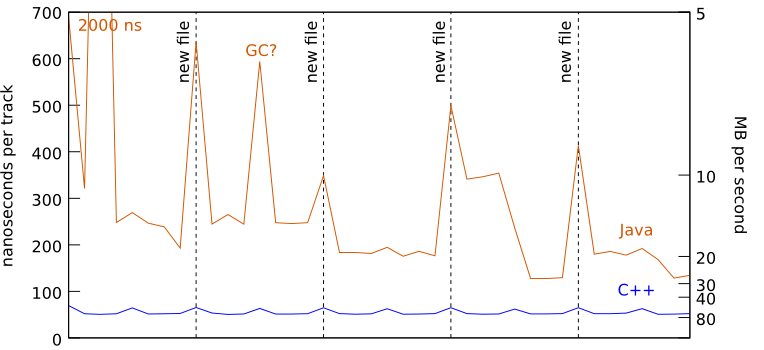
\includegraphics[width=0.8\linewidth]{root4j_reading_tracks.png}
\end{center}

\caption{\label{root4j_reading_tracks} Rate of reading track $\chi^2$ in root4j and C++ ROOT as a function of time. (Samples on the horizontal axis are every 100,000 tracks and ``MB'' refers to {\it decompressed} data.)}
\end{figure}

These files were also pre-read before measuring any data, so that they would be in Linux's memory cache, effectively removing the physical bottleneck of disk access and ensuring that neither software product is unfairly discounted because of this large bottleneck.

Both C++ and Java readers are deserializing and decompressing (deflate) the same bytes. The C++ ROOT version is 6.08/04 (pre-built binary for Ubuntu Linux). The root4j version is 0.1-pre2; spark-root and Spark were {\it not} involved in this test (which would complicate matters, due to caching). Both have been executed in a single process, single thread.

In the plot, we see that standard C++ ROOT is consistently faster than root4j. We also see that, unlike C++, root4j starts slow and accelerates. We see the HotSpot optimization phase as a spike (temporary slow-down) at the beginning of reading, a spike when opening each file, and a single spike in the middle of one file read. Spikes like these appear at different times in different runs, so they are likely garbage collector pauses.

However, the asymptotic speed of root4j, which is all that matters for large files and large datasets, is about four times slower than C++. Depending on the user's intended purpose, this cost may be worthwhile, since it opens direct access to all the ``big data'' and machine learning tools that have been developed for the Java platform.

More recent performance benchmarks are in development, using Spark's built-in performance counters\footnote{\href{https://github.com/diana-hep/spark-root/blob/master/md/PerformanceBenchmarksPublicDS.md}{\tt https://github.com/diana-hep/spark-root/blob/master/md/PerformanceBenchmarksPublicDS.md}}.

\section*{ROOT file reading: CMSSW vs optimized C++}

The second test of ROOT file reading was motivated by Femtocode, which takes advantage of ROOT's columnar data representation on disk to perform calculations in the same format in memory, without reconstructing objects. This is in contrast to a traditional framework for analyzing physics data, such as CMSSW.

CMSSW uses ROOT to build instances of C++ classes, and physicist users write C++ code to interact with those objects. Since arbitrary-length collections of record structures ({\tt std::vector<SomeClass>}) are common, these objects may not be contiguous in memory. Since the user code could access any attribute from these classes, all columns associated with the whole class must be loaded, even if the user actually accesses only one or two.

Femtocode, on the other hand, is a high level language that gets JIT-compiled to machine code. Part of this compilation process determines which attributes are needed and only loads those. The code is also compiled in such a way that it runs on contiguous arrays of data loaded directly from the ROOT file without constructing objects first.

Femtocode's strategy is similar to {\tt TTree::Draw}, a special-purpose function for aggregating data into histograms (and immediately drawing them). Femtocode and {\tt TTree::Draw} differ in that Femtocode is JIT-compiled and more general, but the similarities are close enough that a comparison to {\tt TTree::Draw} would be helpful.

Table~\ref{cmssw-table} compares the file-reading performance of CMSSW, {\tt TTree::Draw}, and a ROOT-reading routine designed for Femtocode. This specialized reader uses the ROOT libraries, but avoids function calls that would reconstruct C++ objects from the data, as an ordinary user would want. We thank Philippe Canal for his help in writing this routine.

\begin{table}
\caption{\label{cmssw-table} File-reading rates in events per millisecond per process (kHz per process). In each case, the goal was only to access the $p_T$ (or $E_T$) attribute of each particle, though CMSSW loads all attributes associated with the particle.}

\begin{center}
\begin{tabular}{l c c c c c}
          &\# of particles & \# of attributes & CMSSW &{\tt TTree::} & Femtocode \\
particle  & per event (avg) & (``branches'') & EDAnalyzer &{\tt Draw()} & ROOT reader \\\hline
photon    & 2.9    & 205         & \mbox{\ \ \ \ \ } 1.14 kHz   &   \mbox{\ \ \ \ \ } 435 kHz       &   \mbox{\ \ \ \ \ } 769 kHz \\
electron  & 2.5     & 231         & 1.02   &   417       &   833        \\
muon      & 2.7     & 192         & 1.02   &   16.5      &   770        \\
tau       & 6.3     &  88         & 1.55   &   244       &   417        \\
jet       & 16.7    &  95         & 1.15   &   123       &   182        \\
AK8 jet   & 1.8     &  95         & 2.10   &   556       &   1000       \\
\end{tabular}
\end{center}
\end{table}

The CMSSW reader uses version {\tt 8\_0\_25} of the CMSSW software with a custom EDAnalyzer following current best-practices for file-reading ({\tt EDGetTokenT<>} and {\tt consumes<>} to inform CMSSW of which particles will be loaded). The goal was to extract the $p_T$ (or $E_T$) value from a variety of particles (individually, in separate runs). CMSSW is at a disadvantage for this kind of test because it must load all attributes of the selected particle because it doesn't analyze user code to see which are necessary. The different particle types have 95--231 attributes (called ``branches'' in ROOT), so for this task, CMSSW is reading a hundred times more data than necessary. This roughly correlates with its performance.

(Experiment frameworks like CMSSW were also designed for event reconstruction, which requires many more attributes per particle and has a performance that is closer to optimal.)

The {\tt TTree::Draw} function was designed to plot small numbers of branches, so it does not load unnecessary attributes. Similarly, Femtocode is primarily intended for plotting, so its specialized reader calls a similar set of functions as {\tt TTree::Draw}. In most cases, their results are within a factor of 2 of each other, though the muon comparison is a factor of 50. (This has been reported to the ROOT team; they are investigating.) The factor of 2 can be expected, since {\tt TTree::Draw} is additionally invoking an interpreter to generate a plot, unlike the other readers, which simply add up $p_T$ values (to ensure that it is not eliminated by the compiler).

All tests were single-process, single-thread, reading the same input file that was pre-loaded into Linux cache by previous reads. The {\tt TTree::Draw} tests were rotated in order and the first call was discarded, since {\tt TTree::Draw} does some initialization the first time it is called.

In addition to comparing these three ways of calling ROOT routines to read ROOT files, we tested the time required to read a flat array of the same size from a Numpy file. Numpy files have a very simple format: the contiguous array is compressed (deflate, same as ROOT) and written to disk as-is (with a small header). The Femtocode ROOT reader was only 5\% slower than reading the equivalent data from Numpy files, which suggests that the procedure is near optimal.

\section*{Memory bandwidth: conventional vs GPU vs KNL}

Because of the high cost of loading data into memory, Spark and Femtocode cache that data for subsequent computations. This fits the work-pattern of data analysis, in which a computation is often repeated with subtle variations as part of exploratory data analysis or systematics studies. Assuming that the whole dataset can be loaded, all but the first pass benefit from the cache, often by orders of magnitude (100--1000$\times$).

At these high rates, the bottleneck shifts from disk or network to the DRAM memory. For a sample plotting problem, we performed a simple operation (addition) on 10 billion double-precision floating point numbers. We arrived at this figure because 100 million events is typical of a high energy physics dataset (all $t\bar{t}$ data collected by CMS since its inception is 100~fb$^{-1}$ $\times$ 1~nb = 100 million events) and the plotting code may need to access 100 values per event (hundreds of tracks or combinations of attributes). This is 80~GB of in-memory data to be evaluated while the user waits.

The throughput from DRAM to CPU back to DRAM is highly affected by compiler optimizations, which target this specific problem. Compiling the same loop with {\tt -O0} and {\tt -O3} yields 70~seconds and 13~seconds to process the same data, respectively. (Test performed in a single process, single thread.)

The plotting problem is embarrassingly parallel and can be horizontally scaled to a nearly arbitrary degree, dividing this 13~seconds by a factor of $N$. However, we also wanted to see if specialized hardware could solve the problem. We performed the same simple operation on several different GPUs and one Knight's Landing (KNL) chip. The GPU results are summarized in Table~\ref{gpu-results}: some GPU models have faster memory, some have faster computation, and others are embedded in an architecture with a faster connection to main memory. However, on most architectures, the time required to copy data from DRAM to the GPU was equal to the time required to copy data from DRAM to the CPU: the GPU could be regarded as just as ``distant'' from main memory as the CPU. (Biggest deviation: 60\% slower for GPU.)

\begin{table}
\caption{\label{gpu-results} GHz rates}

\begin{center}
\begin{tabular}{l c c c c c c}
                  &  GeForce & GRID     & Tesla  & Tesla  & Tesla       & Tesla     \\
                  &  GTX     & K520     & K40c   & K20Xm  & K20m        & P100-SXM2 \\
                  &  660M    & (AWS)    & (CERN) & (CERN) & (Princeton) & (CERN)    \\
Data transfers:   &          &          &        &        &             &           \\\hline
DRAM to {\it CPU} & 1.804 1.54557 0.77261 0.773144 0.8192 3.45566       
DRAM to GPU       & 1.69467 0.970904 0.816211 0.507478 0.867488 3.3825  
GPU to DRAM       & 1.69467 0.984867 0.491712 0.759666 0.514087 1.84568 
CPU write unified & 2.3141 1.53427 0.8194 0.495927 0.87177 3.56583      
CPU read unified  & 2.3141 1.50065 0.477507 0.4641 0.498284 2.05477     
within GPU        & 6.99051 15.183 23.6299 23.6299 18.8508 56.8719      
                  &          &          &        &        &             &           \\
Calculations:     &          &          &        &        &             &           \\\hline
in-place global   & 3.99458 13.6957 21.3722 21.1034 16.8615 56.8719
immutable global  & 4.14252 14.2785 21.5093 21.237 16.9467 56.8719 
in-place unified  & 2.62144 2.22362 2.57715 1.61708 1.43579 7.09396
immutable unified & 2.91778 2.39333 2.93822 2.88021 1.54486 8.32616
\end{tabular}
\end{center}
\end{table}



%% milliseconds for 1 GB
%% DRAM to {\it CPU} & 18.6     &    21.71 &  43.43 &  43.40 &       40.96 &      9.71 \\
%% DRAM to GPU       & 19.8     &    34.56 &  41.11 &  66.12 &       38.68 &      9.92 \\
%% GPU to DRAM       & 19.8     &    34.07 &  68.24 &  44.17 &       65.27 &     18.18 \\
%% CPU write unified & 14.5     &    21.87 &  40.95 &  67.66 &       38.49 &      9.41 \\
%% CPU read unified  & 14.5     &    22.36 &  70.27 &  72.30 &       67.34 &     16.33 \\
%% within GPU        &  4.8     &     2.21 &   1.42 &   1.42 &        1.78 &      0.59 \\
%%                   &          &          &        &        &             &           \\
%% Calculations:     &          &          &        &        &             &           \\\hline
%% in-place global   &  8.4     &     2.45 &   1.57 &   1.59 &        1.99 &      0.59 \\
%% immutable global  &  8.1     &     2.35 &   1.56 &   1.58 &        1.98 &      0.59 \\
%% in-place unified  & 12.8     &    15.09 &  13.02 &  20.75 &       23.37 &      4.73 \\
%% immutable unified & 11.5     &    14.02 &  11.42 &  11.65 &       21.72 &      4.03 \\





Another thing worth knowing is that data copies {\it within} the GPU are much faster than copies to or from the GPU.






%% 	GRID K520 (Amazon)	Tesla K40c (CERN)	Tesla K20Xm (CERN)	Tesla K20m (Princeton)	Tesla P100-SXM2 (CERN)	Ratio K20m/P100
%% Data transfers (ms for 1 GB):						
%% Host-to-host copy (no GPU)          	
%% Host-to-device copy             	
%% Device-to-host copy            	
%% Host write to unified memory     	
%% Host read from unified memory	
%% Device-to-device copy one GPU)	
%% Calculations (ms for 1 GB):						
%% In-place operation - x, float32)	
%% Immutable operatio - x, float32)	
%% In-place operation on unified memory	
%% Immutable on unified memory    	


%% Device at 0:
%%     name: 
%%     totalGlobalMem: 1.95135 GB
%%     sharedMemPerBlock: 48 kB
%%     regsPerBlock: 65536
%%     warpSize: 32
%%     memPitch: 2 GB
%%     maxThreadsPerBlock: 1024
%%     maxThreadsDim: 1024 1024 64 
%%     maxGridSize: 2147483647 65535 65535 
%%     totalConstMem: 64 kB
%%     version: 3.0
%%     clockRate: 950 MHz
%%     textureAlignment: 512
%%     deviceOverlap: true
%%     multiProcessorCount: 2
%%     kernelExecTimeoutEnabled: false
%%     integrated: false
%%     canMapHostMemory: true
%%     computeMode: cudaComputeModeDefault
%%     concurrentKernels: true
%%     ECCEnabled: false
%%     pciBusID: 1
%%     pciDeviceID: 0
%%     tccDriver: false

%% 1 GB host -> host: 39.125 ms
%% 1 GB host -> host: 19.982 ms
%% 1 GB host -> host: 19.21 ms
%% 1 GB host -> host: 18.724 ms
%% 1 GB host -> host: 18.611 ms
%% check 0.178395 0.399677 0.166599
%% 1 GB host -> device: 20.019 ms
%% 1 GB host -> device: 19.91 ms
%% 1 GB host -> device: 19.84 ms
%% 1 GB host -> device: 19.89 ms
%% 1 GB host -> device: 19.882 ms
%% 1 GB device in-place operation: 8.413 ms
%% 1 GB device in-place operation: 8.404 ms
%% 1 GB device in-place operation: 8.403 ms
%% 1 GB device in-place operation: 8.405 ms
%% 1 GB device in-place operation: 8.407 ms
%% 1 GB device immutable operation: 7.993 ms
%% 1 GB device immutable operation: 8.064 ms
%% 1 GB device immutable operation: 8.102 ms
%% 1 GB device immutable operation: 8.074 ms
%% 1 GB device immutable operation: 8.164 ms
%% 1 GB device const immutable operation: 8.138 ms
%% 1 GB device const immutable operation: 8.157 ms
%% 1 GB device const immutable operation: 8.14 ms
%% 1 GB device const immutable operation: 8.108 ms
%% 1 GB device const immutable operation: 8.068 ms
%% 1 GB device -> host: 19.639 ms
%% 1 GB device -> host: 20.215 ms
%% 1 GB device -> host: 19.942 ms
%% 1 GB device -> host: 19.895 ms
%% 1 GB device -> host: 19.883 ms
%% check 0.821605 0.600323 0.833401
%% 1 GB host -> pinned: 14.521 ms
%% 1 GB host -> pinned: 15.759 ms
%% 1 GB host -> pinned: 14.868 ms
%% 1 GB host -> pinned: 14.444 ms
%% 1 GB host -> pinned: 14.459 ms
%% 1 GB device in-place operation: 13.111 ms
%% 1 GB device in-place operation: 12.858 ms
%% 1 GB device in-place operation: 12.82 ms
%% 1 GB device in-place operation: 12.895 ms
%% 1 GB device in-place operation: 13.192 ms
%% 1 GB device immutable operation: 11.851 ms
%% 1 GB device immutable operation: 12.297 ms
%% 1 GB device immutable operation: 11.521 ms
%% 1 GB device immutable operation: 11.57 ms
%% 1 GB device immutable operation: 11.509 ms
%% 1 GB device const immutable operation: 11.5 ms
%% 1 GB device const immutable operation: 12.468 ms
%% 1 GB device const immutable operation: 11.549 ms
%% 1 GB device const immutable operation: 12.297 ms
%% 1 GB device const immutable operation: 12.189 ms
%% 1 GB pinned -> host: 14.434 ms
%% 1 GB pinned -> host: 15.915 ms
%% 1 GB pinned -> host: 15.032 ms
%% 1 GB pinned -> host: 14.492 ms
%% 1 GB pinned -> host: 14.516 ms
%% check 0.178395 0.399677 0.166599
%% 1 GB device -> device: 5.058 ms
%% 1 GB device -> device: 4.831 ms
%% 1 GB device -> device: 4.829 ms
%% 1 GB device -> device: 4.829 ms
%% 1 GB device -> device: 4.831 ms




\end{document}
